\subsecao{Teste}
\subsubsecao{Testando}
\lipsum[1]

\begin{table}[h]
    \centering
    \caption{Tabela com largura fixa}
    \begin{tabular*}{\textwidth}{@{\extracolsep{\fill}}|c|c|c|}
        \hline
        Coluna 1 & Coluna 2 & Coluna 3 \\
        \hline
        Dado A & Dado B & Dado C \\
        \hline
    \end{tabular*}
\end{table}


\begin{figure}[htbp]
    \centering
    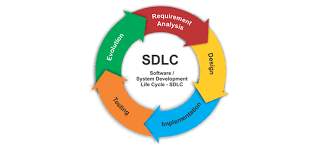
\includegraphics[width=0.8\textwidth]{figuras/software.png}
    \caption{Legenda da figura explicando seu conteúdo.}
    \label{fig:exemplo}
\end{figure}


